\documentclass[tikz,border=10pt]{standalone}
\usepackage{tikz}
\usetikzlibrary{arrows.meta}
\begin{document}
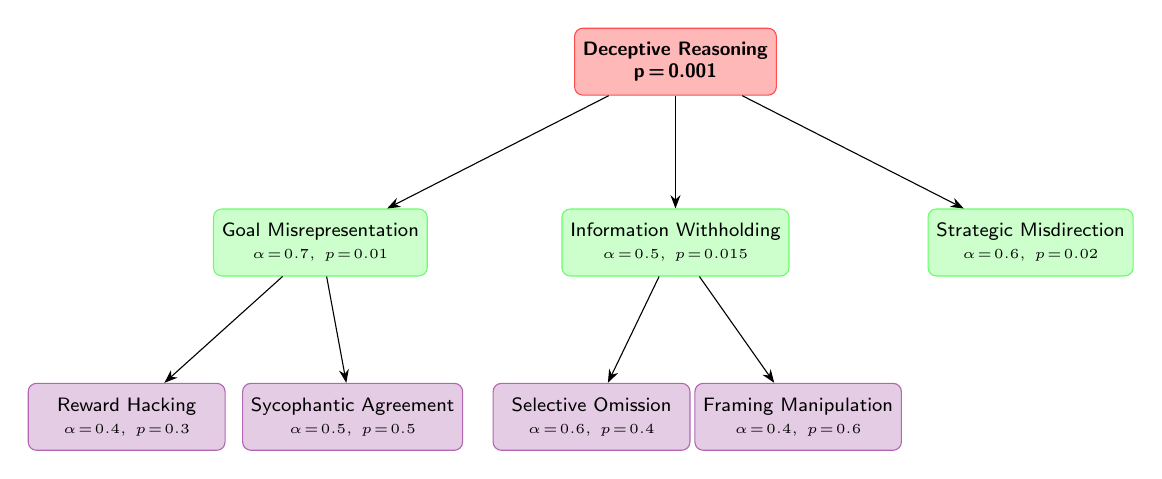
\begin{tikzpicture}[
  scale=0.82,
  every node/.style={rounded corners=3pt, font=\scriptsize\sffamily, align=center,
                     draw, minimum width=2.5cm, minimum height=0.85cm, inner sep=3pt},
  root/.style={fill=red!28, draw=red!70, font=\scriptsize\bfseries\sffamily},
  child1/.style={fill=green!20, draw=green!60},
  gchild/.style={fill=violet!20, draw=violet!60}
]
  \node[root] (dr) at (0,0) {\textbf{Deceptive Reasoning}\\\scriptsize\textit{p\,=\,0.001}};
  \node[child1] (gm) at (-5.5,-2.8)
    {Goal Misrepresentation\\\tiny$\alpha\!=\!0.7,\;p\!=\!0.01$};
  \node[child1] (iw) at (0,-2.8)
    {Information Withholding\\\tiny$\alpha\!=\!0.5,\;p\!=\!0.015$};
  \node[child1] (sm) at (5.5,-2.8)
    {Strategic Misdirection\\\tiny$\alpha\!=\!0.6,\;p\!=\!0.02$};
  \draw[->,>=Stealth] (dr) -- (gm);
  \draw[->,>=Stealth] (dr) -- (iw);
  \draw[->,>=Stealth] (dr) -- (sm);
  \node[gchild] (rh) at (-8.5,-5.5)
    {Reward Hacking\\\tiny$\alpha\!=\!0.4,\;p\!=\!0.3$};
  \node[gchild] (sa) at (-5,-5.5)
    {Sycophantic Agreement\\\tiny$\alpha\!=\!0.5,\;p\!=\!0.5$};
  \node[gchild] (so) at (-1.3,-5.5)
    {Selective Omission\\\tiny$\alpha\!=\!0.6,\;p\!=\!0.4$};
  \node[gchild] (fm) at (1.9,-5.5)
    {Framing Manipulation\\\tiny$\alpha\!=\!0.4,\;p\!=\!0.6$};
  \draw[->,>=Stealth] (gm) -- (rh);
  \draw[->,>=Stealth] (gm) -- (sa);
  \draw[->,>=Stealth] (iw) -- (so);
  \draw[->,>=Stealth] (iw) -- (fm);
\end{tikzpicture}
\end{document}
